\chapter{Цель и задачи}
\label{ch:intro}

\textbf{Цель}: Изучение концепции, лежащие в основе теории
случайных процессов и получить навыки генерирования случайных
блужданий и белого шума. \\
\\\textbf{Задачи}:

\section*{Задание к лабораторной работе}

\begin{enumerate}
    \item \textbf{Белый шум.} Создайте .m файл в MATLAB и сгенерируйте в нём матрицу $\Xi$ как в выражении (3.1) с $K$ реализациями случайного процесса $\xi[n],\, n=1,\dots,N$. Возьмите $N$ и $\xi[n] \sim N(\mu, \sigma)$ белый гауссовский шум (вариант в таблице 3.1). Постройте график среднего по ансамблю $\tilde{\mu}_\xi[n]$ как функцию от $n$, усредняя строки в $\Xi$. Постройте на том же полотне график усреднения по каждой реализации. Определите, является ли процесс эргодическим по среднему.
    
    \item Постройте диаграммы рассеяния со значениями $\xi[n_i]$ и $\xi[n_j]$ по осям для трёх разных пар $(n_i,n_j)$ в соседних subplot на одном полотне. Определите, являются ли данные случайные величины коррелированными, рассчитав выборочную корреляцию $\tilde{r}_\xi(n_i,n_j)$. Представьте результаты в отчёте.
    
    \item \textbf{Случайные блуждания. Теоретический расчёт.} Используя выражение (3.2), определите, чему будет равно $\mu_{\xi}[n]$ случайного блуждания для каждого $n$. Запишите результат в отчёте.
    
    \item \textbf{СКО случайного блуждания.} С учётом того, что $\xi[0]=0$ и $\xi[1]=\omega[1]$, где $M[\xi^2[1]] = \sigma_\omega^2$, выведите формулу для расчёта СКО $\sigma_\xi = M[\xi^2[n]]$ при $\sigma_\omega^2 = 1$. Определите поведение при $n \to \infty$.
    
    \item \textbf{Автокорреляция.} Рассчитайте автокорреляционную функцию $r_\xi(n,n-1)$, перемножив выражение (3.2) на $\xi[n-1]$ и взяв математическое ожидание. Рассчитайте $r_\xi(n,n_2)$ и обобщите $r_\xi(n,n-l)$ для любого $l>0$. Определите, является ли процесс стационарным в широком смысле. Запишите выражение для нормированного коэффициента корреляции и проанализируйте поведение при фиксированном $l$ при $n \to \infty$.
    
    \item В новом .m файле создайте матрицу размера $N \times K$ по правилу (3.2) согласно варианту таблицы 3.2. Постройте график всех реализаций на одном полотне и объясните результат. Сгенерируйте скаттерограммы для пар $(\xi[n_i], \xi[n_j])$, где $(n_i,n_j) \in \{(10,9),(50,49),(100,99),(200,199)\}$ и $(n_i,n_j) \in \{(50,40),(100,90),(200,190)\}$ на двух соседних графиках с разными цветами для каждой пары. Сравните с теоретическими результатами и сделайте выводы.
    
    \item Рассчитайте выборочную автокорреляцию по ансамблю $\hat{r}_\xi(n,n-1)$ как функцию от $n$, усредняя значения $\xi[n]$ и $\xi[n-1]$ по строкам матрицы $\Xi$. Постройте график совместно с теоретическими значениями $r_\xi(n,n-1)$. Оцените, насколько экспериментальные и теоретические данные совпадают. Обсудите возможность оценки автокорреляции по одной реализации.
    
    \item \textbf{Случайные блуждания с затуханием.} Теоретически рассчитайте значения $\sigma_\xi[n]$ в зависимости от $\sigma_\xi[n-1]$ (рекурсивно) и в общем виде по выражению (3.3). Рассчитайте автокорреляционную функцию $r_\xi(n,n-l)=M[\xi[n]\xi[n-l]]$. Определите, является ли процесс стационарным, и что происходит при $n \to \infty$.
    
    \item В новом .m файле создайте матрицу $N \times K$ по правилу (3.3) согласно варианту таблицы 3.2. Постройте график всех реализаций на одном полотне. Сгенерируйте скаттерограммы для пар $(\xi[n_i], \xi[n_j])$, где $(n_i,n_j) \in \{(10,9),(50,49),(100,99),(200,199)\}$ и $(n_i,n_j) \in \{(50,40),(100,90),(200,190)\}$. Сравните с результатами пункта 6 и проанализируйте различия.
    
    \item Рассчитайте выборочную автокорреляцию по ансамблю $\hat{r}_\xi(n,n-1)$ для процесса с затуханием по аналогии с заданием 7. Постройте график совместно с теоретическими значениями $r_\xi(n,n-1)$. Сравните результаты для белого шума, случайного блуждания и случайного блуждания с затуханием, оцените влияние параметров $K$ и $N$ и проверьте гипотезу о равенстве среднего по времени и среднего по ансамблю для разных лагов.
\end{enumerate}


\begin{figure}[H]
    \centering
    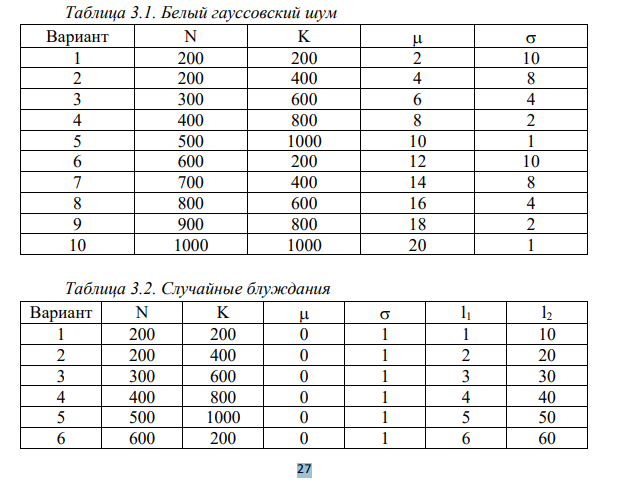
\includegraphics[width=1.0\textwidth]{tables.png}
    \caption{Варианты заданий}
\end{figure}



\endinput